\section{Evaluation}
\label{OBS:Sec:Evaluation}

\begin{figure*}[ht]
        \centering
        \subfigure[$\mathcal{R}_1$, packets received per host in $net_1(d=2, f=3)$] {
                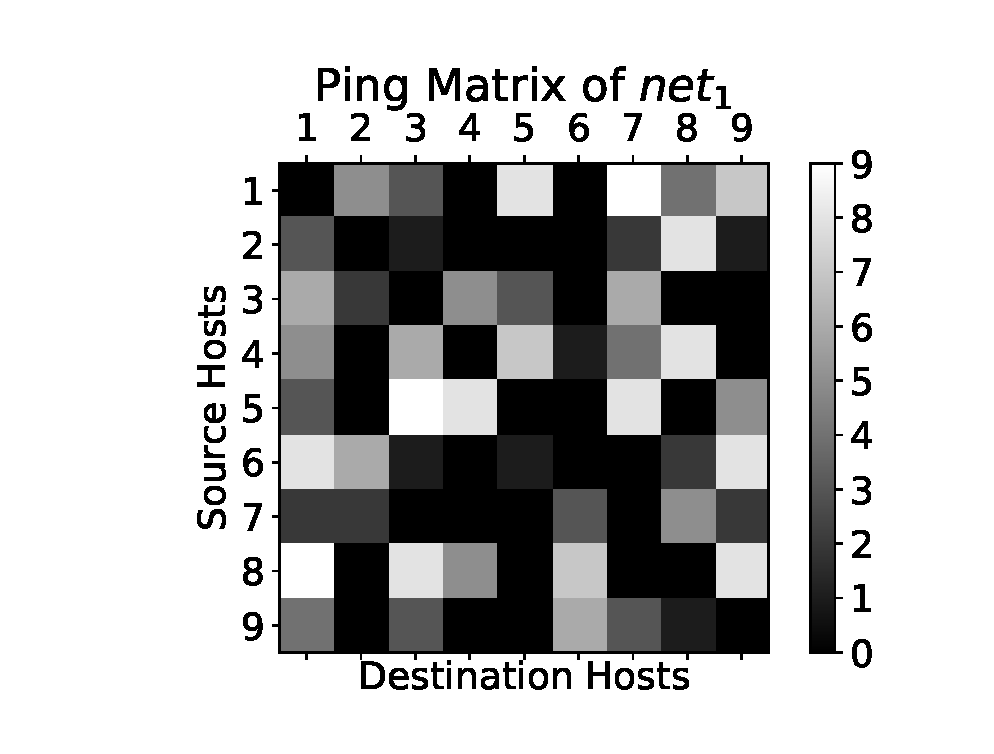
\includegraphics[width=.45\textwidth]{OneBigSwitch/figures/ping_mat_2_3.eps}
                \label{OBS:Fig:PingMatrix1}
        }
        \subfigure[$\mathcal{R}_2$, Packets received in $net_2(d=2, f=3)$] {
                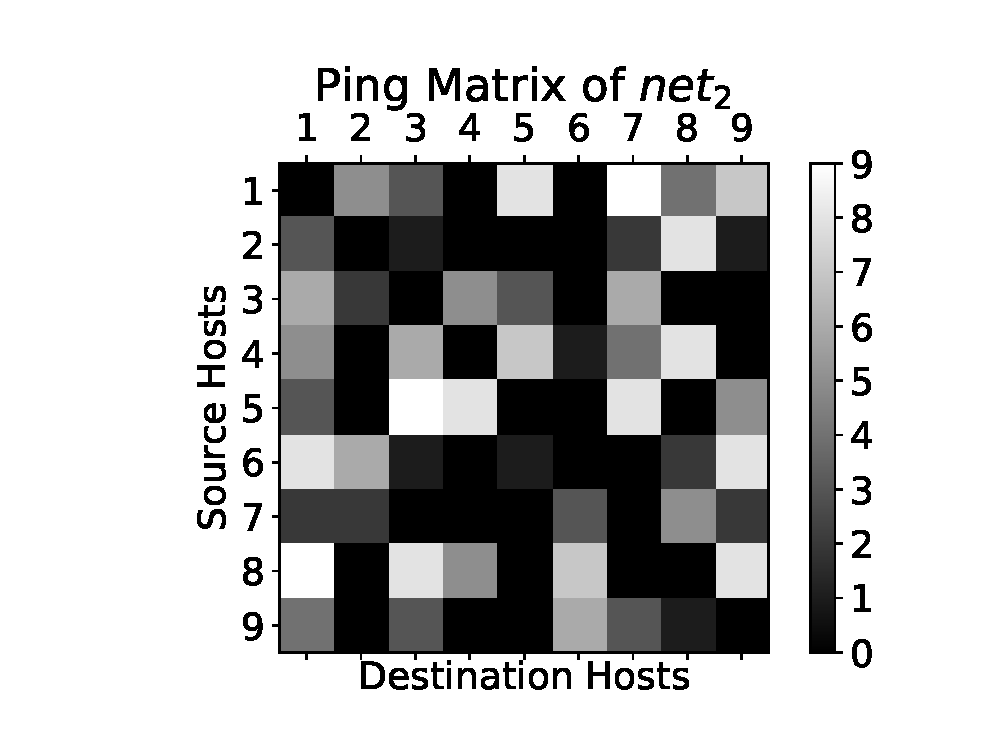
\includegraphics[width=.45\textwidth]{OneBigSwitch/figures/bs_ping_mat_2_3.eps}
                \label{OBS:Fig:PingMatrix2}
        }
        \\
        \subfigure[$\mathcal{R}_1$, Packets received in $net_1(d=4, f=3)$] {
                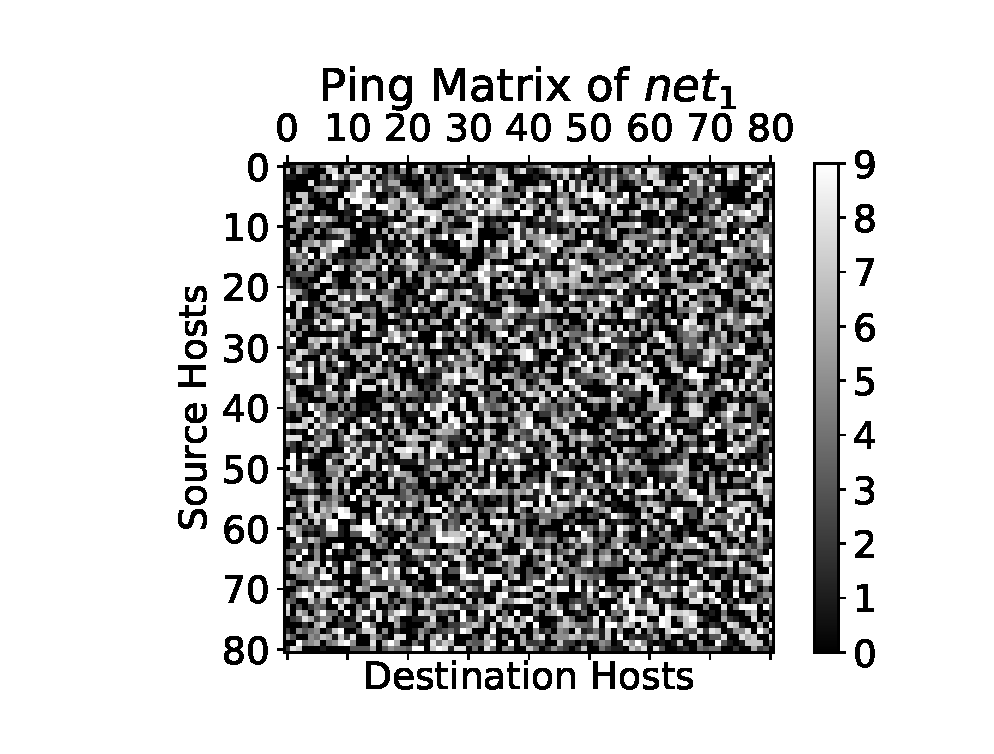
\includegraphics[width=.45\textwidth]{OneBigSwitch/figures/ping_mat_4_3.eps}
                \label{OBS:Fig:PingMatrix3}
        }
        \subfigure[$\mathcal{R}_2$, Packets received in $net_2(d=4, f=3)$] {
                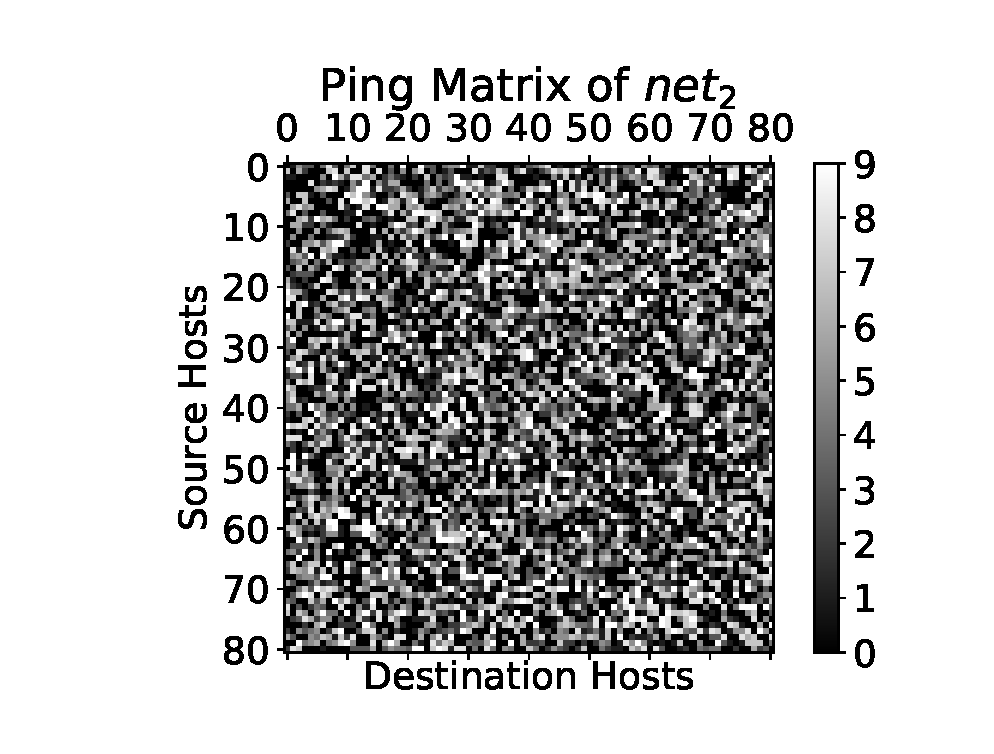
\includegraphics[width=.45\textwidth]{OneBigSwitch/figures/bs_ping_mat_4_3.eps}
                \label{OBS:Fig:PingMatrix4}
        }
        \caption[Forwarding Logic Evaluation after One-Big-Switch Abstraction]{
        Matrix $\mathcal{R}$ represents the number of packets received at each host.
        $net_1$ is the original SDN network with a tree topology ($d$, $f$),
        where $d$ is depth and $f$ is fanout.
        $net_2$ is the corresponding one-big-switch-based network.
        The gradient legend visualizes the number of received packets.
        $\mathcal{R}_1$ and $\mathcal{R}_2$ are identical,
        which indicate that our model abstraction technique preserves the network forwarding logic.}
        \label{OBS:Fig:ComparePingMatrix}
\end{figure*}

\begin{figure}[ht]
\centering
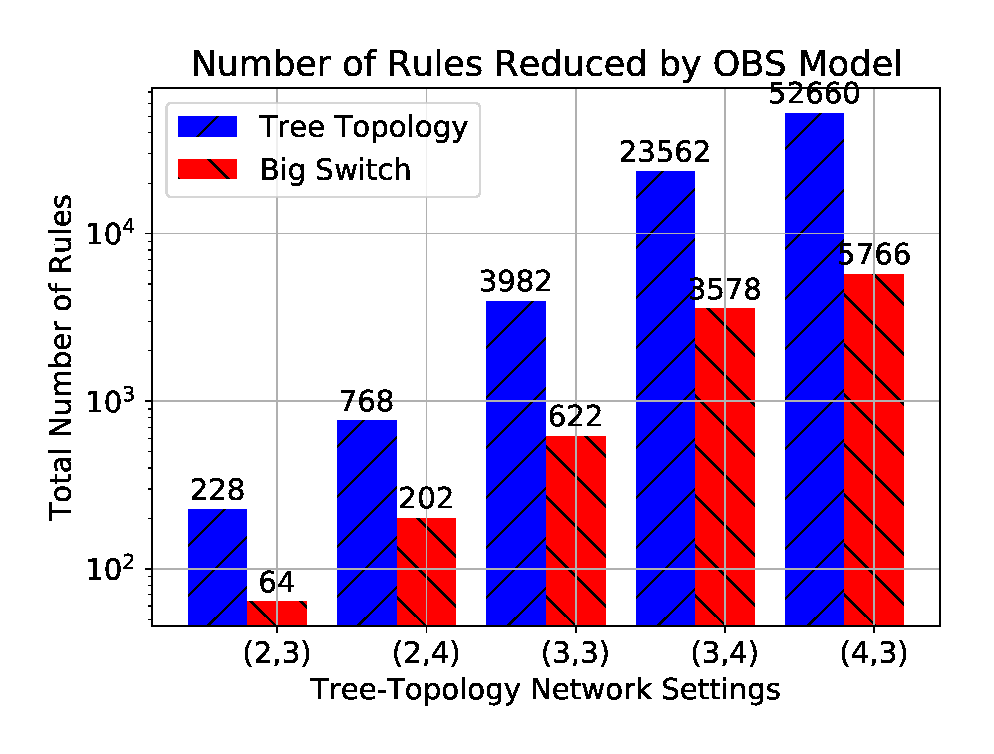
\includegraphics[width=0.9\textwidth]{OneBigSwitch/figures/comp_num_rules.eps}
\caption[Number of Rules Reduced after One-Big-Switch Abstraction]{Number of rules needed to preserve the network forwarding logic.
        The number of rules on the big switch is about 72\% to 89\% less than
        the number of rules in the original tree-topology network.
        The x-axis label ($d$, $f$) represents the depth and fanout parameters
        in a tree topology network.}
\label{OBS:Fig:CompareNumRules}
\end{figure}


\begin{figure}[ht]
\centering
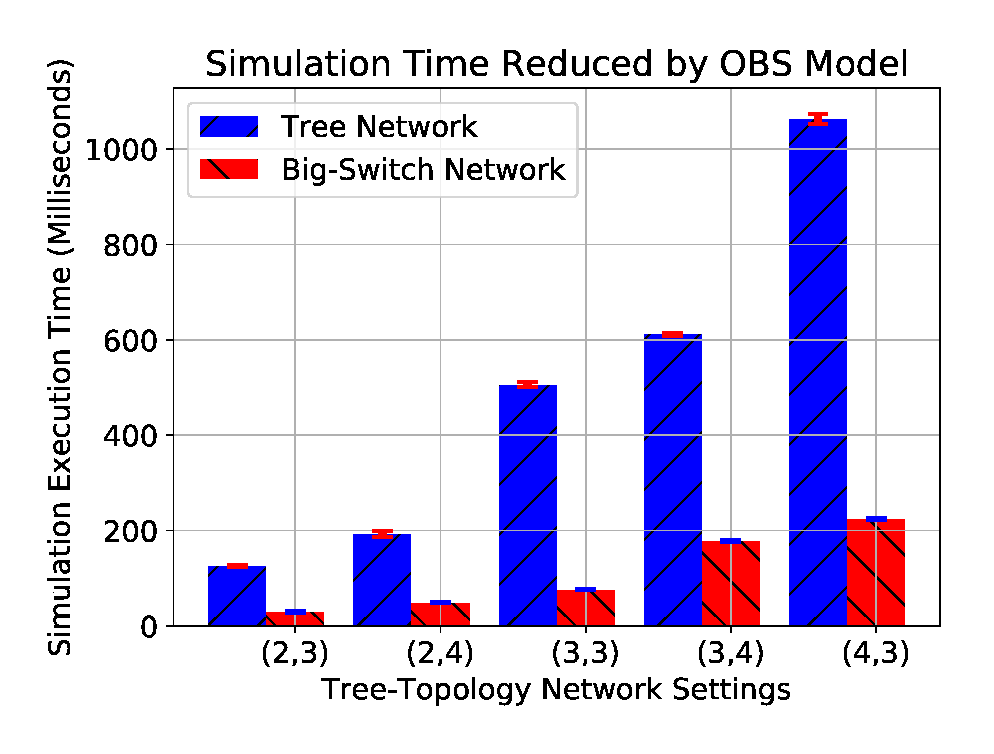
\includegraphics[width=0.9\textwidth]{OneBigSwitch/figures/comp_sim_time.eps}
\caption[Comparison of Simulation Execution Time]{Comparison of simulation execution time.
        The big-switch-based network model saves about 75\% to 85\% running time
        as compared to simulating the corresponding SDN-based network.
        The x-axis label ($d$, $f$) represents the depth and fanout parameters in a tree topology network.}
\label{OBS:Fig:CompareSimulationTime}
\end{figure}

\begin{figure}[ht]
\centering
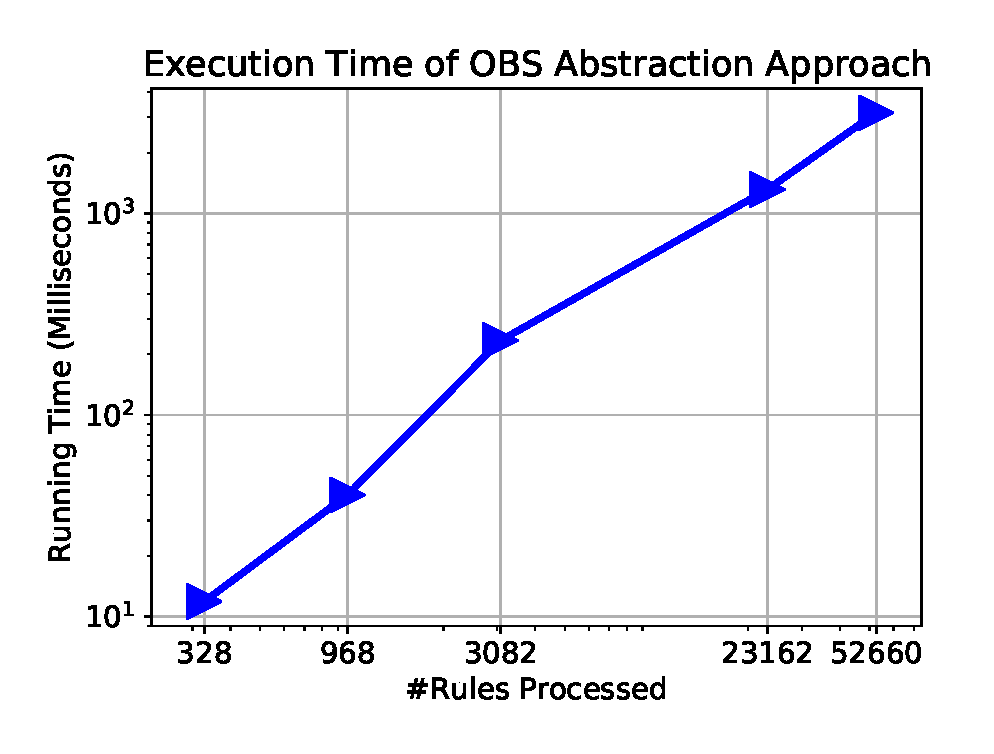
\includegraphics[width=0.9\textwidth]{OneBigSwitch/figures/bs_overhead.eps}
\caption[Execution Time of One-Big-Switch Abstraction]{Execution time to transform an SDN-based network to a big-switch-based network.}
\label{OBS:Fig:BSOverhead}
\end{figure}

\subsection{Network Forwarding Logic Equivalence}
\label{OBS:SubSec:PreserveForwardingLogic}
We perform experimental evaluation of our network model abstraction technique
that transforms an SDN-based network to one-big-switch model.
The evaluation results show that our approach significantly saves simulation/emulation resources
(e.g., number of forwarding rules) and simulation execution time,
while still preserving the forwarding behavior of the original network.

Our experiments simulate and emulate networks of type tree topology.
The tree network is described by two topological parameters: depth $d$ and fanout $f$.
Such network $tree(d, f)$ can connect $f^d$ hosts with $\frac{f^d - 1}{f-1}$ switches in total.
%Though not known as a scalable network architecture (a good scalable alternative will be fat-tree topology), it is good for demonstration purpose since the tree topology is well-structured and
All end-hosts in a tree network are fully-connected with at most $2d$ hops.


We first demonstrate that the forwarding logic of the original software-defined network is exactly preserved by the abstracted big-switch model.
%One can find the shortest path between a pair of hosts $(s, d)$ with a layer-two learning switch controller application. Traversing the tree up and down in breadth-first-search style, learning switch application can automatically install OpenFlow rules on each hop once we initiate \texttt{ping} between the given pair of host. More specifically,
\if 0
\hl{
Since the production SDN network snapshot, including topology connections and rules installed on
individual switches, are not easy to obtain, our demonstration is based on the following plausible setup.
}
\fi
We created a tree-topology network $net_1$ in Mininet~\cite{Mininet},
and connected all the switches to an SDN controller running a layer-two learning switch application~\cite{Pox}.
%We generated the network forwarding rules by establishing communication paths between random selected host pairs.
%For any network host $s$, we randomly generate a list of distinct hosts $dsts$, and let $s$ \texttt{ping} each host $dst \in dsts$.
After performing the \texttt{ping} tests between randomly selected pairs of end-hosts,
the controller application generated all the network forwarding rules and installed them on the switches.
We then took a snapshot of the network, including (1) the host-to-switch and switch-to-switch connections,
and (2) the rules on all the switches using the \texttt{ovs-ofctl dump-flows} command. The snapshot was used to generate the rules for the big-switch model as well as the port mapping according to the algorithms presented in Section~\ref{OBS:Sec:Design}.

We then created another emulated network $net_2$ in Mininet, consisting of one OpenFlow switch and the same number of hosts as $net_1$.
The switch was connected to $f^d$ hosts with the port numbers derived from both the $PortMap$ (Algorithm~\ref{OBS:Alg:GenAllRules})
and the link information ($net_1$'s topology).
The rules generated by Algorithm~\ref{OBS:Alg:GenAllRules} were installed on the switch using the \texttt{ovs-ofctl add-flow} command.

To validate that the big-switch-network preserved the network forwarding logic of the original network,
we recorded the connectivity between \emph{every} host pair in both $net_1$ and $net_2$,
and compared the results.
Specially, the original network $net_1$ is a tree network with $f^d$ hosts,
where $d$ is the depth and $f$ is the fanout of a tree network.
Each host sent a number of \texttt{ping} packets to every other host in $net_1$,
and the amount of packet was randomly selected between 1 and 10.
We repeated the experiments in $net_2$ with the same traffic pattern.
The result was represented in a matrix $\mathcal{R}$,
where $\mathcal{R}[i][j]$ denotes the numbers of successfully received \texttt{ping}
packets from host $i$ to host j, where $i \neq j$, and $i, j \in [1, f^d]$.

%To prevent l2\_learning switch controller from installing new rules in $net_1$, we take down the pox controller in this stage.
%The result of this experiment is a matrix $\mathcal{R}_k$ where $\mathcal{R}[i][j]$ denote

We repeated the experiment for different combinations of $d$ and $f$, i.e., ($d, f$) $\in$
\{(2, 3), (2, 4), (3, 3), (3, 4), (4, 3)\}. For each network scenario,
we saved the experimental results in $\mathcal{R}_1$ and $\mathcal{R}_2$, and compared the two matrices using the \texttt{diff} command.
We found that $\mathcal{R}_1 = \mathcal{R}_2$ holds true for all five network scenarios.
We visualized $\mathcal{R}_1$ and $\mathcal{R}_2$ for the ($d=2, f=3$) and ($d=4, f=3$) cases
in Figure~\ref{OBS:Fig:ComparePingMatrix}.
We can see that the original SDN-based network and the abstracted one-big-switch-based
network have the identical network forwarding logic,
measured by the connectivity and the number of receiving packets for each connection.
%In Figure~\ref{Fig:PingMatrix1}-Figure~\ref{Fig:PingMatrix4},
Note that the brightness of the element in the matrix is proportional to $\mathcal{R}[i][j]$,
i.e., the number of successfully delivered packets from host $i$ to host $j$.
%It is easy to see that $\mathcal{R}_1$ and $\mathcal{R}_2$ are identical for all experiment settings.

\subsection{Performance Gain}

\textbf{Number of OpenFlow Rules.} We compare the total number of rules installed
on the switches in both $net_1$ and $net_2$ with the same experimental settings
in Section~\ref{OBS:SubSec:PreserveForwardingLogic}.
The results are plotted in Figure~\ref{OBS:Fig:CompareNumRules} for networks with
various topological parameter settings.
%Note that y-axis is in log scale.
The number of rules needed to preserve the forwarding logic is significantly
less in the one-big-switch-based network as compared with the original SDN-based network
for all scenarios in the range of 71.93\% to 89.05\% reduction.
%approximately one degree of magnitude less than the number of rules existing in the original tree-topology network.
For example, in the case of a network with depth = 4, and fanout = 3, 52,660 rules
in the original network were reduced to 5,766 rules in the big-switch-based network.


\textbf{Simulation Time.}
Our approach significantly reduces network simulation model complexity in terms of
the number of switches and the number of rules.
A key benefit is to reduce the time to run simulation experiments.

We performed the same set of experiments on a network simulator, S3FNet~\cite{S3F}.
We simulated two SDN-based networks: one models a tree-topology network $net_1(d, f)$,
and the other models the corresponding big-switch-based network $net_2$.
We set half of the hosts as TCP clients and the other half as TCP servers,
and conducted one-to-one communication among them.
We sent each traffic flow for 100 seconds in simulation time.
We repeated each experiment ten times and recorded the simulation execution time for both $net_1$ and $net_2$ in
Figure~\ref{OBS:Fig:CompareSimulationTime} for comparison.
The error bars indicate the standard deviations of the running time
for all ten independent simulation runs.
We can see that simulating the big-switch-based network is 3.42 to 6.68 times
faster than simulating the original SDN-based network.


\subsection{Model Abstraction Execution Time}
We discussed the asymptotic time complexity of our model abstraction technique in 
Section~\ref{OBS:Sec:Design}.
We now evaluate the execution time for transforming an SDN-based network to a big-switch-based network.
We recorded the running time for converting various tree networks,
i.e., ($d, f$) $\in$ \{(2, 3), (2, 4), (3, 3), (3, 4), (4, 3)\} in Figure~\ref{OBS:Fig:BSOverhead}.
We can see that the model abstraction process is lightweight.
For example, it took about 40 milliseconds to abstract a small tree network ($d=4$, $f=2$);
for a medium-scale medium-scale tree network (depth 4 and fanout 3),
it took about 3.15 seconds to process 52,660 rules.
The fast model abstraction execution time is useful.
As the network state keeps evolving, it is essential to constantly update the abstracted big-switch model to reflect the changes, preferably in an online fashion.
In fact, the three-step approach allows us to incrementally update the big-switch model and requires far less execution time, i.e.,
we only need to update a small set of rules that are different in the new network snapshot.
